\chapter{Estat actual}
\label{cap:estat}




* Mineria sèries temporals
  
  - mineria
  - aplicacions


* Obtenció de sèries temporals i problemes

  - censura
  - mostreig


* SGBD
 - model relacional
 - implementacions

    - SGBD+xarxes
    - Per sèries temporals

  % * Sèries temporals (històrics, predicció, diagnosis, prognosis, etc.)
  % * Mostreig: docs quan període de mostreig no regular
  % * Bases de dades (docs d'emmagatzematge quan la memòria és finita, docs quan període de mostreig no és regular, altres sistemes semblants (comercials,prototips))



This paper focuses on Data Base Management Systems (DBMS) that store
and treat data as time series.  Traditional DBMS, as is ones derived
from relational model, are not adequate for these cases as they do not
have enough facilities to manage and retrieve time series
information \parencite{schmidt95}.

Some DBMS have already taken into account the specificities of time
series, then called Time Series Data Base Management Systems
(TSMS) \parencite{dreyer94}.  Time Series Data
Server \parencite{weigel10} allows to select a data range from a time
series and to apply a filter when the data is retrieved.
RRDtool \parencite{rrdtool} applies filters and stores different data
ranges when data is stored, moreover it considers that the sampling
times can not be equally spaced, the temporal order is essential and
the value and time must be stored together. However, this TSMS lack
the complete definition of the relation between the three main fields
involved: time series, monitoring systems and DBMS.




DBMS are based from formal models that define the objects and
operations of the abstract machine to which users interact, such is
the relational model \parencite{date}. TSMS lack a consolidated formal
model, although special properties and requirements for a TSMS
have been proposed \parencite{dreyer94}.

In this paper
a model is proposed for an storage system that will keep a time series
in a multiresolution and bounded way.  In this first proposal there
are six definitions that are related to the data storage mechanism:
measure, time series, buffer, disc, resolution disc, and multiresolution
database. Some of this concepts are familiar with RRDtool
operating mode.

En aquest capítol se situen els sistemes de gestió de bases de dades (SGBD) per sèries temporals en el context de la mineria de dades de sèries temporals (\emph{time series data mining}), el qual també es considerat com mineria de dades per  detectar automàticament coneixement (\emph{knowledge discovery databases}). Els SGBD de model Round Robin (RRD) pertanyen a aquest context ja que  emmagatzemen sèries temporals  de les quals es vol aconseguir informació rellevant.

El capítol comença resumint l'estat de les sèries temporals en aquest camp de mineria; és a dir d'emmagatzematge i tractament. A continuació es llisten algunes aplicacions informàtiques que han implementat models de la mineria de sèries temporals. Finalment, es descriu l'estat actual de l'aplicació RRDtool, la qual també es classifica en aquest camp.





\section{Sèries temporals}

Important! Diferència entre dades temporals i sèries temporals.




Obtaining information from environment is a complex task that has a user, either human or machine, as the final target as stated in figure \ref{fig:sistema_monitoratge}.
 Mainly, the processes between data acquisition and user information can be divided into three focus.


Monitoring systems recollect data from sensors eventually from events and periodically from measures, in the latter case some problems arise when monitoring can not be done at regular intervals. Then the recollected data is used in different application fields. There is intensive research in applying techniques to obtain information from this data.

Time series data mining analyses the storage of chronological data from which relevant information want to be retrieved. Sometimes, this extraction of information is also referred as knowledge discovery or artificial intelligence.
In the monitoring context, the data collected can be considered as a time series.

Database management systems are the computer systems implementing storage and retrieval of information. Time series data mining techniques must be implemented in these systems paying attention to their especial needs. Then, they are known as time series database management systems.








\subsection{Mineria de sèries temporals}

La mineria de sèries temporals (\emph{time series data mining}) és el procés d'anàlisis i descobriment de patrons en sèries temporals. És un camp recent que acompanya els processos de descobriment de coneixement a les bases de dades (\emph{knowledge discovery in databases}) \parencite{last01}.


La recerca en mineria de sèries temporals s'ha incrementat en la darrera dècada tal com esmenta \textcite{fu11} en un article recent. L'objectiu principal és reduir la mida de les sèries temporals per tal de processar amb menor temps les dades.
\citeauthor{fu11} resumeix l'estat actual de la mineria de sèries temporals de forma exhaustiva i conclou que encara queden molts problemes per investigar i resoldre. La recerca en tasques de mineria ha estat intensa però es necessita millorar la representació de sèries temporals, ja que es considera el pas que redueix la mida de les dades. A més a més, les sèries temporals es consideren un dels deu problemes prioritaris  en la mineria de dades \parencite{yangwu06}.

Segons \textcite{keogh02}, les quatre tasques que centren l'atenció de la recerca actual de sèries temporals són l'indexat (\emph{indexing}), l'agrupament (\emph{clustering}), la classificació (\emph{classification}) i la segmentació (\emph{segmentation}). A més, \citeauthor{keogh02} comparen  alguns algoritmes experimentals duts a terme en aquests camps per diversos autors. Recomanen a la comunitat de mineria de sèries temporals que segueixi el seu estudi com a punt de referència per avaluar el rendiment d'algoritmes similars.

Un pas comú previ a les quatre tasques anteriors és el de representació de la sèrie temporal. 
La representació de sèries temporals a trossos lineals (PLR, \emph{Piecewise Linear Representation}) \parencite{keogh97,keogh98} {é}s la més habitual actualment per ser més propera als usuaris ja que la visió de l'ésser humà segmenta les corbes en línies rectes.
Després de definir la PLR, \textcite{keogh00,keogh01} exploren altres representacions de sèries temporals per tal de reduir la dimensió d'una sèrie temporal i poder-la indexar més fàcilment. Proposen dues tècniques eficients en el càlcul: la \emph{Piecewise Aggregate Aproximation} i la \emph{Adaptive Piecewise Constant Approximation}, ambdues basades en la representació a trossos constants de la sèrie temporal. 
D'aquestes dues tècniques, \citeauthor{keogh00,keogh01} conclouen que mantenen una bona aproximació a la sèrie temporal i que a més  tenen molt menys cost de càlcul que altres de més complicades, com ara la \emph{Discrete Fourier Transform},  la  \emph{Singular Value Decomposition} o la \emph{Discrete Wavelet Transform}.




\subsubsection{Aplicacions de les sèries temporals}

L'anàlisi de sèries temporals abasta camps molt diferents com ara la predicció econòmica, la medicina, la meteorologia, la qualitat industrial, etc. En aquest context,  la mineria de sèries temporals tracta de gestionar co\l.leccions cronològiques de dades que tenen una mida gran i que contínuament estan en creixement.


L'ús de sèries temporals per analitzar les dades té com a objectius la comprensió del comportament de les variables observades, poder trobar-ne un model d'ajust i utilitzar-lo per a predicció o per a llaços de control.


El monitoratge de dades de sensors i el processat de les dades per tal d'aconseguir diagnosis, prognosis, predicció, fusió de dades i altres tasques d'anàlisi de sèries temporals són comunes en diferents camps com ara prognosis en models de degradació \parencite{yu11}, qualificació de l'estat dels sensors en vaixells \parencite{palmer07}, validació i reconstrucció de dades en xarxes de distribució d'aigua \parencite{quevedo10}, classificació de valors econòmics \parencite{dreyer95}, optimització de la planificació semafòrica \parencite{last11} o estimació del temps de viatge en autopistes \parencite{soriguera10}.



Un dels camps recents on la mineria de sèries temporals hi té molta aplicació és en les xarxes de sensors. L'abaratiment del maquinari permet monitorar el procés amb grans quantitats de sensors inte\l.ligents \parencite{jainagrawal05,gehrkemadden04}, els quals tenen processador i ràdio incorporats però tenen recursos limitats pel que fa a transmissió, energia i processat. Així doncs, el problema  de les xarxes de sensors rau en estudiar l'ús eficient d'aquests recursos, pel qual actualment trobem dues propostes.
Una solució consisteix en transmetre la informació a un node central comprimint-la tant amb agregacions com amb aproximacions \parencite{deligiannakis07}.
Una altra solució consisteix en tenir les dades distribuïdes en diferents sensors i quan es llança una consulta es decideix a on s'ha de resoldre, el qual s'anomena xarxa de sensors amb sistema distribuït de base de dades \parencite{gehrkemadden04}.


\subsection{Monitoratge de sèries temporals}

Els sistemes de monitoratge són un part important del control i interacció amb els processos. Principalment, aquests sistemes s'encarreguen de recollir dades, conèixer l'estat actual del procés i informar a l'usuari. Els sistemes de monitoratge constitueixen la part principal dels sistemes SCADA (\emph{Supervisory Control And Data Acquisition}). Un SCADA  és el sistema encarregat de recollir i centralitzar les dades de manera periòdica en el temps.



\begin{figure}[tp]
  \begin{center}
    \scriptsize 
    \usetikzlibrary{arrows,positioning}
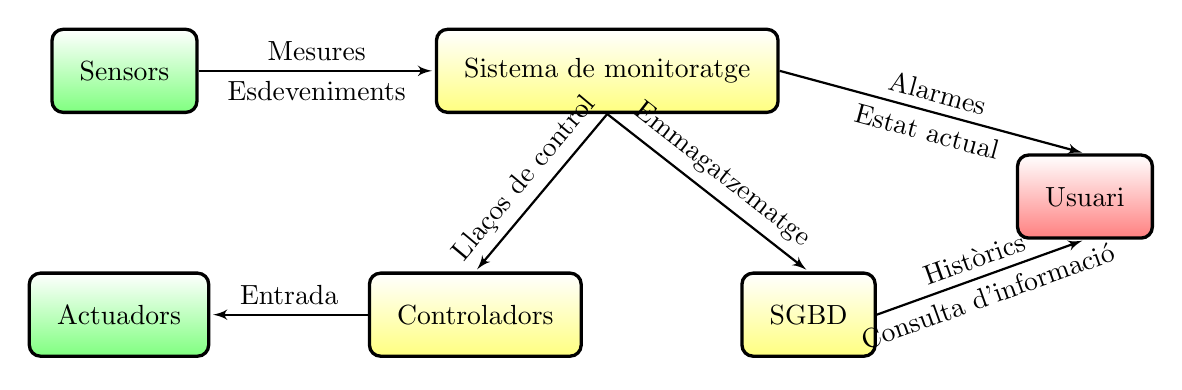
\begin{tikzpicture}[node distance=0.5cm]  
  \tikzset{
    mynode/.style={rectangle,rounded corners,draw=black, 
      very thick, inner sep=1em, minimum size=3em, text centered,
      groc},
    myarrow/.style={->, >=latex', shorten >=1pt, thick},
    mylabel/.style={text width=7em, text centered},
    groc/.style={top color=white, bottom color=yellow!50},
    verd/.style={top color=white, bottom color=green!50},
    roig/.style={top color=white, bottom color=red!50},
  }  

  \node[mynode]                                       (monitor)   {Sistema de monitoratge};  
  \node[mynode, below right=2cm and -0.5cm of monitor]  (bd)        {SGBD}; 
  \node[mynode, below=2cm of monitor, left=2cm and 2cm of bd]     (control)   {Controladors}; 
  \node[mynode, roig, below right=0.5cm and 3cm of monitor] (usuari)    {Usuari};  
  \node[mynode, verd, left=2cm of control]            (actuador)  {Actuadors};
  \node[mynode, verd, left=3cm of monitor]            (sensor)    {Sensors};  


  \draw[myarrow] (monitor.east) --   (usuari.north)	
     node [above,sloped,midway] {Alarmes}
     node [below,sloped,midway] {Estat actual};
  \draw[myarrow] (bd.east) --   (usuari.south)
     node [above,sloped,midway] {Històrics}
     node [below,sloped,midway] {Consulta d'informació};
  \draw[myarrow] (sensor.east) --   (monitor.west) 
     node [above,midway] {Mesures}
     node [below,midway] {Esdeveniments};
  \draw[myarrow] (control.west) -- (actuador.east)
     node [above,midway] {Entrada};
  \draw[myarrow] (monitor.south) -- (bd.north)
     node [above,sloped,midway] {Emmagatzematge};
  \draw[myarrow] (monitor.south) -- (control.north)
     node [above,sloped,midway] {Llaços de control};

\end{tikzpicture} 
  \end{center}
  \caption{Sistema de monitoratge: de l'adquisició de dades fins a informar l'usuari}
  \label{fig:sistema_monitoratge}
\end{figure}


El monitoratge es pot dividir en diferents blocs principals, els quals es mostren a la \autoref{fig:sistema_monitoratge}. Un monitor adquireix dades dels sensors. Les dades poden ser valors de mesures o estats del procés adquirits com a esdeveniments. 

Per una banda, les dades es poden utilitzar com a sortida del procés en els sistemes de control, els quals calculen els valors d'entrada dels accionaments.
Els llaços de control poden no estar tan centralitzats i habitualment resideixen a prop dels processos que controlen.

Per altra banda, els sistemes de monitoratge informen l'usuari de l'estat actual del procés, tot i que poden només avisar-lo amb alarmes senzilles com per exemple que no s'han pogut adquirir les dades o que el sensor ha disparat un esdeveniment crític. Per a usuari ens referim tant a un usuari humà com a un altre sistema supervisor amb inte\l.ligència artificial. 

Per a càlculs més complicats amb les dades, els sistemes de monitoratge utilitzen sistemes de gestió de bases de dades (SGBD). Mitjançant els SGBD, s'emmagatzemen les dades en bases de dades i posteriorment l'usuari les consulta per observar els històrics o per obtenir informació i descobrir coneixement a partir de les dades emmagatzemades.




\subsubsection{Problemes en el monitoratge}

Els sistemes de monitoratge habitualment reben problemes derivats de la reco\l.lecció de dades. Principalment distingim tres problemes.

El primer problema és la gestió d'una quantitat enorme de dades. 

Un sistema de monitoratge recull una gran quantitat de dades. Ara bé, l'usuari només en pot observar una petita part sincronitzat (\emph{online}) amb el procés i les dades emmagatzemades esdevenen massa grans per a ser processades posteriorment \parencite{keogh97}. No obstant, les dades han de ser analitzades ja que contenen informació interessant per a les aplicacions de les sèries temporals descrites a l'apartat anterior. S'observa que en el context de monitoratge les dades recollides es poden considerar com a sèries temporals ja que abstractament són una co\l.lecció de mesures.


El segon problema és el de la necessitat de censurar les dades, és a dir validar que les dades siguin correctes i en cas contrari rebutjar-les o reconstruir-les. 

\textcite{quevedo10} mostren la quantitat d'informació que hi ha en els sistemes complexos de telecontrol. Aquesta informació s'obté de diversos sensors distribuïts pel camp de mesura.
En el moment de reco\l.lecció de dades apareixen dos problemes: valors que en un instant de temps prefixat no s'han pogut recollir i valors que són falsos. En el procés de gestió de dades no es poden emmagatzemar les dades amb aquests dos tipus de problema ja que aleshores els registres històrics serien inconsistents. 
Així doncs, cal comprovar que les dades emmagatzemades són correctes, mitjançant un procés de validació, i modificar-les en el cas que siguin falses, mitjançant un procés de reconstrucció que estimi els valors correctes. Per exemple, \citeauthor{quevedo10} apliquen aquests processos de validació i reconstrucció a xarxes de distribució d'aigua.


El tercer problema és dóna quan el període de mostreig no és regular, és a dir que les dades no es recullen de manera uniforme en el temps, però les aplicacions no ho contemplen o volen treballar amb dades a intervals regulars, també anomenat dades equi-espaiades.

Una causa de la irregularitat es deu a que els sistemes de monitoratge informàtics sovint no són capaços de complir amb exactitud el temps de mesura sinó que presenten una certa variació, ja sigui deguda a retards en els sensors, les comunicacions o la planificació del monitoratge amb altres tasques concurrents del sistema operatiu. Aquesta causa, però, es pot atenuar si els sensors envien el temps de mesura juntament amb el valor mesurat.

Una altra causa es deu a que l'adquisició de dades prové de processos sotmesos a sistemes de control, els quals prenen el control de l'adquisició de dades. És a dir, el sistema de monitoratge ha d'obeir a les restriccions de temps imposades pels llaços de control. Aquestes restriccions són especialment crítiques en els sistemes de control en temps real ja que, aleshores, el sistema de monitoratge no pot imposar restriccions de temps diferents de les que s'han calculat per als llaços de control.  \textcite{lozoya08} mostren que s'ha de vigilar amb les entrades i sortides de les tasques periòdiques als sistemes en temps real. L'actuació dels sistemes de control es degrada quan no es té en compte que les operacions d'entrada i sortida estan subjectes a fluctuacions degudes al mostreig i a latències. Aquest problema afecta als sistemes de monitoratge en dues vessants.
Per una banda, els sistemes de monitoratge tenen una part de l'adquisició controlada per les aplicacions de control en temps real i per tant el període de mostreig resultant que veu el monitor no és regular. 
Per altra banda, les aplicacions que analitzen les dades obtingudes del monitoratge poden veure com la seva actuació es degrada si no consideren que l'adquisició de dades és irregular, el qual és similar a la regressió que s'observa quan en el disseny d'un controlador discret es considera que es mostreja i s'actua periòdicament però en la implementació amb un sistema en temps real aquest pot fluctuar la periodicitat \parencite{lozoya08}.




En conclusió, per tal de gestionar la complexitat derivada de la recollida de dades i també la complexitat de les consultes posteriors per part de l'usuari, els sistemes de monitoratge es recolzen en sistemes de gestió de bases de dades per gestionar l'emmagatzematge de les dades i la recuperació d'informació.




\subsection{SGBD per sèries temporals}

ficar aquí els sgbd per sèries temporals i més endavant ja es parlarà dels sgbd en general i com modelar-los i implementar-los.


\subsubsection{cougar}

cougar databases

http://www.cs.cornell.edu/bigreddata/cougar/index.php




                                                                 At
                   Berkeley and Cornell, we’ve built two prototype
                   sensor network query processors (SNQPs)—
                   TinyDB (http://telegraph.cs.berkeley.edu/tinydb)
                   and Cougar (http://cougar.cs.cornell.edu)—that
                   run on a variety of sensor platforms. \parencite{gehrkemadden04}





\section[SGBD]{Sistemes de gestió de bases de dades}

Els sistemes de gestió de bases de dades (SGBD) 



L'any 1970 (i 1969) Codd va proposar un model relacional pels SGBD (SGBDR) que va revolucionar aquest àmbit. A partir de llavors els SGBDR han anat evolucionat, amb Date com a principal divulgador, fins a tenir una gran solidesa.

Avui dia, no hi cap implementació comercial que segueixi fidelment el model relacional \todo{citar date}, tot i que n'hi ha que caminen cap aquest camí (rel,TransRelational). Això ha contribuït a que per una banda hi hagi hagut una sèrie de malentesos i errors que Date s'ha encarregat de desmentir en nombroses publicacions \todo{citar, sobretot ddbunk} i per altra banda també ha contribuït en gran mesura a voler explorar altres models.              


Alguns SQL squirks (the possibility of nulls, the possibility of duplicate rows, the
fact of left-to-right column ordering, and so on), tema modernament discutit són els nulls [datesigmod2008]

Alguns malentesos també es deuen en l'ús de la mateixa terminologia amb significat diferent entre el model relacional i l'orientació a objectes, sobretot pel que fa als termes valor i variable. 

Relacional: tipus | representació |  valor, objecte, instància  | variable  | referència (adreça continguda en una variable) | operadors (de lectura i de modificació)
Objectes: tipus, classe (tipus amb atributs i mètodes), interfície | classe, atributs,propietats  |  valor, estat, objecte/instància immutable/estàtic |  valor, objecte/instància mutable/dinàmic  | variable | funcions,mètodes (funcions dins de classes) (purs o modificadors)

Aquesta confusió pot ser deguda a 'the object model' is closer to being a model of storage than it is to being a model of data. [date06]


Hi han hagut algunes propostes per apartar-se del model relacional, com pot ser recuperant models antics de xarxa (Xquery) o bé utilitzant el paradigma de programació d'objectes \todo{cites}, tot i que Date i altres consideren que no estan ben fundades i cap d'aquestes té la mateixa potència que el model relacional. Actualment s'està treballant en una implementació fidel al model relacional \todo{citar}. 

Date i altres consideren la possibilitat, tot i que remota, que es pugui definir un model més potent que el relacional però que no hi ha cap indici que cap definició ho estigui aconseguint ni de fet explorant. Per tant, aconsellen que cap aplicació de gestió de bases de dades no s'allunyi del model relacional.


El model relacional es basa en la lògica de predicats i la teoria de conjunts.





Com s'ha d'estendre el model relacional?

Date i altres consideren que el model relacional va evolucionat i no consideren que hi hagi hagut cap revolució des de la seva aparició. (Tot i que han definit una nova àlgebra relacional anomenada 'A' que fa molt bona pinta). Consideren que el model relacional està bastant completat i l'evoluciona en petites modificacions de comprensió. 

Només hi ha hagut un àmbit en el que han admès que s'havia d'estendre el model relacional i aquest és el de les dades temporals \todo{citar}.  'Support for interval-valued attributes (and hence for temporal databases) involves among other things support for
%generalized versions of the usual relational operators.' [date]            Note: Those “U_” operators are all defined in terms of two new relational operators called pack and unpack,
and those latter operators in turn are defined in terms of relation-valued attributes. As already noted, therefore, support
for interval-valued attributes relies on support for relation-valued attributes, at least conceptually. 




Així doncs no hi ha necessitat d'estendre el model relacional. Sí que hi ha necessitat, però, de tenir disponibles diversos tipus de dades. La creació de nous tipus de dades ha estat un tema de molta confusió ja que les 'suposades' implementacions del model relacional no ho han permès, o les extensions proposades per \textcite{stonebraker86} es consideren que són a nivell d'implementació i no les que es desitjarien a nivell de model, i sobretot ha fet que les implementacions basades en orientació a objectes tinguessin un gran impacte \todo{citar ODMG (object databases)}. Date ha rebutjat aquesta idea argumentant que el model relacional mai no ha fixat els tipus de dades disponibles sinó que ben al contrari mai n'ha parlat i per tant els tipus de dades han tingut total llibertat de creació; si bé el model relacional defineix que com a mínim hi ha d'haver el tipus booleà i el tipus relació.

El model relacional requereix que hi hagi un 'sistema' de tipus però diu molt poc de la naturalesa d'aquest sistema de tipus; això es coneix com a ortogonalitat entre les relacions i els tipus.



Així doncs, tenint en compte que segons Date el model relacional és complet, que no hi ha cap de tant potent i que l'ampliació de funcionalitat dels SGBDR s'ha de fer mitjançant la creació de nous tipus, el SGST hauria de contemplar aquestes idees. 

Primer s'hauria de veure que el cas de les sèries temporals no sigui com el cas de les dades temporals a on sí que s'ha necessitat estendre el model relacional.

Segon, s'hauria de considerar que el SGST són un nou tipus de dades en el model relacional i per tant el model relacional ja té tota la potència per una banda constituir SGBD i per altra banda definir i incorporar nous tipus.


Com es defineixen nous tipus complexos als SGBD?

En el cas que es descarti que el cas dels SGST presenta els mateixos problemes que les dades temporals i per tant els SGST han d'esdevenir un tipus de dades, cal preguntar-se com són els tipus de dades al model relacional.

Concretament el model relacional només defineix què es un tipus de dades però dóna llibertat a la seva creació. Això és un gran avantatge. En els cas de tipus de dades senzills es defineixen amb una bona estructura i ja està però què passa quan es vol definir un nou tipus de dades complex?

Cal recercar com s'han definit nous tipus de dades complexos. Els principals problemes es donen que el tipus és complex i forma una entitat de per sí. És a dir que definir un tipus sèrie temporal no és trivial. Aleshores, com cal procedir?



Sobre la necessitat de modelar els tipus.

Cal definir un model pel tipus que volem dissenyar.
De fet, volem dissenyar un SGST. És a dir, un tipus que conformi pròpiament un SGBD. Per tant, utilitzarem les mateixes eines que es fan servir per modelar els SGBDR per a poder modelar el nostre SGST. Com que s'hauran utilitzat les mateixes eines, el SGST podrà esdevenir perfectament un tipus de dades pels SGBDR.

En resum, per a definir nous tipus complexes cal modelar-los com a entitat pròpia, fent un símil amb el model relacional. Això no vol dir, però, que un cop modelats constitueixin de per sí un nou model per als SGBD, sinó que queden dins dels SGBDR. \todo{caldria} elaborar més i trobar alguna pista de com definir nous tipus complexos, stonebraker86 només indica com es va estendre postgresql amb operadors de creació de nous tipus però no com s'han de modelar els nous tipus.

Volem crear un nou model de SGBD, Date ens diu que només hi ha el model relacional, per tant hem d'utilitzar el model relacional per a definir el nostre nou model.




\subsection{Sobre implementació i model}

Diferència entre implementació i model segons Date. Això aporta independència de dades; molt important: els models no han de tenir detalls d'implementació ni parlar d'objectius de rendiment.
Actualment hi ha certa confusió sobre la independència entre el model i la implementació, com es veu tot seguit.


Recentment ha aparegut un nou corrent en l'àmbit dels SGBD que s'anomena NoSQL (Not Only SQL). Diuen que volen sobrepassar les limitacions dels SGBD relacionals. Crec que aquí hi ha un malentès, deuen voler dir sobrepassar les limitacions de les implementacions comercials del model relacional, moltes vegades referides com a SQL pel llenguatge de consulta que utilitzen. En alguns casos a NoSQL es confon implementació amb model ja que es parla de que NoSQL millora el rendiment dels SGBD però en el model mai es parla de rendiment. 

És més, en Date es posiciona en contra de SQL per ser una mala implementació del model relacional, i ha desenvolupat el llenguatge TutorialD que precisament no és SQL. 


Tornant a NoSQL, aquest no genera cap conflicte amb el model relacional. Sovint NoSQL critiquen els SGBD relacionals per voler ser 'one size fits all' \parencite{stonebraker07,stonebraker09} però que cada aplicació té els seus requisits i per tant una mateixa implementació no pot ser bona per a tots el camps. El model relacional no hi pot estar més d'acord amb aquesta afirmació: un model, infinites implementacions. Així doncs aquí hi ha el malentès per culpa de les implementacions errònies de SQL. El model relacional continua sent vàlid i admet qualsevol implementació: ha admès durant anys les denominades SQL, a les quals ha criticat per ser males implementacions, i ara pot admetre les NoSQL. En principi, el model relacional, per ser un model de 'tots' els SGBD, també descriu els productes NoSQL.

No obstant, caldria observar si els productes NoSQL pateixen el mateix mal que els SQL: fer una mala implementació del model relacional. TuotialD és, o pretén ser, una implementació completa del model relacional tot i que a nivell acadèmic.
Ara bé, una implementació d'un SGBD que vulgui  obtenir un bon rendiment en una determinada aplicació potser no pot implementar el model relacional complet sinó que només una part; aleshores aquesta implementació no es pot anomenar SGBD relacional? És a dir, a què s'anomena SGBD relacional? -Un que es pot modelar amb el model relacional: tots(en el moment actual)? -Un a on l'usuari hi veu clarament els conceptes del model relacional.

Actualment sembla que la comunitat informàtica s'ha centrat en les implementacions (garantir propietats ACID, no garantir-les, optimització de consultes, emmagatzematge de grans volums de dades, consultes via web, bases de dades distribuïdes, gastar el mínim d'energia, etc.) \parencite{stonebraker07,stonebraker10}, la qual cosa és excel·lent per a disposar un SGBD adequat a cada aplicació i per tant ha de continuar treballant en aquest camí. Ara bé, sembla que ha oblidat que hi ha un model, el relacional, que descriu com ha de ser un SGBD per a obtenir la màxima potència de cara a la gestió de dades per part de l'usuari i que encara no s'ha trobat cap altre model que tingui la mateixa potència. 







\section{Preguntes}

El llenguatge dels SGBD, per exemple D, és declaratiu (what) i no procedural/imperatiu (how). Com lliguen els SGBD amb els llenguatges de programació declaratius, per exemple amb la programació lògica amb Prolog? Concretament, com lliga Prolog amb el concepte de SGBD? Té la mateixa potència un SGBD que Prolog?
 Es pot veure Prolog com un SGBD?

http://stackoverflow.com/questions/2117651/difference-between-sql-and-prolog





%%% Local Variables: 
%%% mode: latex
%%% TeX-master: "main"
%%% End: 

% LocalWords:  monitoratge
